% Options for packages loaded elsewhere
% Options for packages loaded elsewhere
\PassOptionsToPackage{unicode}{hyperref}
\PassOptionsToPackage{hyphens}{url}
\PassOptionsToPackage{dvipsnames,svgnames,x11names}{xcolor}
%
\documentclass[
  10pt,
]{article}
\usepackage{xcolor}
\usepackage[paper=letterpaper,top=1.3cm,bottom=1.7cm,left=1.5cm,right=1.5cm]{geometry}
\usepackage{amsmath,amssymb}
\setcounter{secnumdepth}{-\maxdimen} % remove section numbering
\usepackage{iftex}
\ifPDFTeX
  \usepackage[T1]{fontenc}
  \usepackage[utf8]{inputenc}
  \usepackage{textcomp} % provide euro and other symbols
\else % if luatex or xetex
  \usepackage{unicode-math} % this also loads fontspec
  \defaultfontfeatures{Scale=MatchLowercase}
  \defaultfontfeatures[\rmfamily]{Ligatures=TeX,Scale=1}
\fi
\usepackage{lmodern}
\ifPDFTeX\else
  % xetex/luatex font selection
\fi
% Use upquote if available, for straight quotes in verbatim environments
\IfFileExists{upquote.sty}{\usepackage{upquote}}{}
\IfFileExists{microtype.sty}{% use microtype if available
  \usepackage[]{microtype}
  \UseMicrotypeSet[protrusion]{basicmath} % disable protrusion for tt fonts
}{}
\makeatletter
\@ifundefined{KOMAClassName}{% if non-KOMA class
  \IfFileExists{parskip.sty}{%
    \usepackage{parskip}
  }{% else
    \setlength{\parindent}{0pt}
    \setlength{\parskip}{6pt plus 2pt minus 1pt}}
}{% if KOMA class
  \KOMAoptions{parskip=half}}
\makeatother
% Make \paragraph and \subparagraph free-standing
\makeatletter
\ifx\paragraph\undefined\else
  \let\oldparagraph\paragraph
  \renewcommand{\paragraph}{
    \@ifstar
      \xxxParagraphStar
      \xxxParagraphNoStar
  }
  \newcommand{\xxxParagraphStar}[1]{\oldparagraph*{#1}\mbox{}}
  \newcommand{\xxxParagraphNoStar}[1]{\oldparagraph{#1}\mbox{}}
\fi
\ifx\subparagraph\undefined\else
  \let\oldsubparagraph\subparagraph
  \renewcommand{\subparagraph}{
    \@ifstar
      \xxxSubParagraphStar
      \xxxSubParagraphNoStar
  }
  \newcommand{\xxxSubParagraphStar}[1]{\oldsubparagraph*{#1}\mbox{}}
  \newcommand{\xxxSubParagraphNoStar}[1]{\oldsubparagraph{#1}\mbox{}}
\fi
\makeatother


\usepackage{longtable,booktabs,array}
\newcounter{none} % for unnumbered tables
\usepackage{calc} % for calculating minipage widths
% Correct order of tables after \paragraph or \subparagraph
\usepackage{etoolbox}
\makeatletter
\patchcmd\longtable{\par}{\if@noskipsec\mbox{}\fi\par}{}{}
\makeatother
% Allow footnotes in longtable head/foot
\IfFileExists{footnotehyper.sty}{\usepackage{footnotehyper}}{\usepackage{footnote}}
\makesavenoteenv{longtable}
\usepackage{graphicx}
\makeatletter
\newsavebox\pandoc@box
\newcommand*\pandocbounded[1]{% scales image to fit in text height/width
  \sbox\pandoc@box{#1}%
  \Gscale@div\@tempa{\textheight}{\dimexpr\ht\pandoc@box+\dp\pandoc@box\relax}%
  \Gscale@div\@tempb{\linewidth}{\wd\pandoc@box}%
  \ifdim\@tempb\p@<\@tempa\p@\let\@tempa\@tempb\fi% select the smaller of both
  \ifdim\@tempa\p@<\p@\scalebox{\@tempa}{\usebox\pandoc@box}%
  \else\usebox{\pandoc@box}%
  \fi%
}
% Set default figure placement to htbp
\def\fps@figure{htbp}
\makeatother





\setlength{\emergencystretch}{3em} % prevent overfull lines

\providecommand{\tightlist}{%
  \setlength{\itemsep}{0pt}\setlength{\parskip}{0pt}}



 


\usepackage[table,dvipsnames]{xcolor}
\usepackage{fontspec}
\setmainfont{Times New Roman}
\usepackage{graphicx}
\usepackage{tabularx}
\usepackage{array}
\usepackage{enumitem}
\usepackage{tcolorbox}
\tcbuselibrary{skins}
\usepackage{fancyhdr}

% ----- 10Power brand palette (sampled from official logo) -----
\definecolor{tpteal}{HTML}{56A8A3}
\definecolor{tporange}{HTML}{E08226}
\definecolor{tpdark}{HTML}{55626F}
\definecolor{tpgray}{HTML}{6B7886}
\definecolor{tplight}{HTML}{EAF4F3}

% ----- layout -----
\setlength{\parindent}{0pt}
\setlength{\parskip}{4pt}
\newcommand{\sep}{\,\textcolor{tpgray}{\textbar}\,}

% ----- arrow bullet list -----
\newlist{arrows}{itemize}{1}
\setlist[arrows]{leftmargin=1.3em,itemsep=2.5pt,topsep=2pt,parsep=0pt,
  label={\textcolor{tporange}{\small$\blacktriangleright$}}}

% ----- feature card -----
\newtcolorbox{featbox}[1]{
  colback=tplight, colframe=tpteal, boxrule=0.6pt, arc=2pt,
  left=7pt, right=7pt, top=4pt, bottom=5pt,
  title={#1}, fonttitle=\bfseries, coltitle=white, colbacktitle=tpteal}

% ----- spec-table helpers -----
\newcommand{\spechead}[1]{\multicolumn{2}{@{}l@{}}{%
  \cellcolor{tpteal}\textcolor{white}{\bfseries\strut\quad #1}}\\}
\newcommand{\tbd}{\textcolor{tporange}{\itshape[to confirm]}}

% ----- footer -----
\pagestyle{fancy}
\fancyhf{}
\renewcommand{\headrulewidth}{0pt}
\renewcommand{\footrulewidth}{0.4pt}
\fancyfoot[L]{\footnotesize\textcolor{tpgray}{\textcopyright\ 2026 New Energy Solutions Lab LLC \sep 10Power}}
\fancyfoot[C]{\footnotesize\textcolor{tpgray}{STREET-EMS Datasheet (DRAFT)}}
\fancyfoot[R]{\footnotesize\textcolor{tpgray}{\thepage}}
\makeatletter
\@ifpackageloaded{caption}{}{\usepackage{caption}}
\AtBeginDocument{%
\ifdefined\contentsname
  \renewcommand*\contentsname{Table of contents}
\else
  \newcommand\contentsname{Table of contents}
\fi
\ifdefined\listfigurename
  \renewcommand*\listfigurename{List of Figures}
\else
  \newcommand\listfigurename{List of Figures}
\fi
\ifdefined\listtablename
  \renewcommand*\listtablename{List of Tables}
\else
  \newcommand\listtablename{List of Tables}
\fi
\ifdefined\figurename
  \renewcommand*\figurename{Figure}
\else
  \newcommand\figurename{Figure}
\fi
\ifdefined\tablename
  \renewcommand*\tablename{Table}
\else
  \newcommand\tablename{Table}
\fi
}
\@ifpackageloaded{float}{}{\usepackage{float}}
\floatstyle{ruled}
\@ifundefined{c@chapter}{\newfloat{codelisting}{h}{lop}}{\newfloat{codelisting}{h}{lop}[chapter]}
\floatname{codelisting}{Listing}
\newcommand*\listoflistings{\listof{codelisting}{List of Listings}}
\makeatother
\makeatletter
\makeatother
\makeatletter
\@ifpackageloaded{caption}{}{\usepackage{caption}}
\@ifpackageloaded{subcaption}{}{\usepackage{subcaption}}
\makeatother
\usepackage{bookmark}
\IfFileExists{xurl.sty}{\usepackage{xurl}}{} % add URL line breaks if available
\urlstyle{same}
\hypersetup{
  colorlinks=true,
  linkcolor={blue},
  filecolor={Maroon},
  citecolor={Blue},
  urlcolor={Blue},
  pdfcreator={LaTeX via pandoc}}


\author{}
\date{}
\begin{document}


% ===================== PAGE 1 : HERO =====================
\thispagestyle{fancy}

% ---- brand header ----
\begin{minipage}[c]{0.55\textwidth}
\IfFileExists{TEN-POWER-LOGO-1.png}{%
  
\includegraphics[height=1.25cm]{TEN-POWER-LOGO-1.png}}{%
  {\fontsize{22}{24}\selectfont\bfseries\color{tpdark}10\color{tpteal}POWER}}
\end{minipage}\hfill
\begin{minipage}[c]{0.43\textwidth}
\raggedleft
\IfFileExists{nesl_logo.png}{
\includegraphics[height=0.75cm]{nesl_logo.png}\\[3pt]}{}
{\footnotesize\textcolor{tpgray}{PRODUCT DATASHEET}}\ \ {\bfseries\color{tpdark}X\textcolor{tporange}{-}EMS}\ {\footnotesize\textcolor{tpgray}{SERIES}}
\end{minipage}

\vspace{3pt}
\textcolor{tporange}{\rule{\textwidth}{2pt}}
\vspace{9pt}

% ---- title + tagline ----
{\fontsize{30}{32}\selectfont\bfseries\color{tpdark}STREET\textcolor{tpteal}{-}EMS}\\[3pt]
{\large\color{tpteal}\itshape Front-of-Meter Feeder Control for the Village Minigrid Street Cabinet}

\vspace{10pt}

% ---- two columns ----
\begin{minipage}[t]{0.60\textwidth}
\IfFileExists{street-ems.jpg}{%
  \begin{center}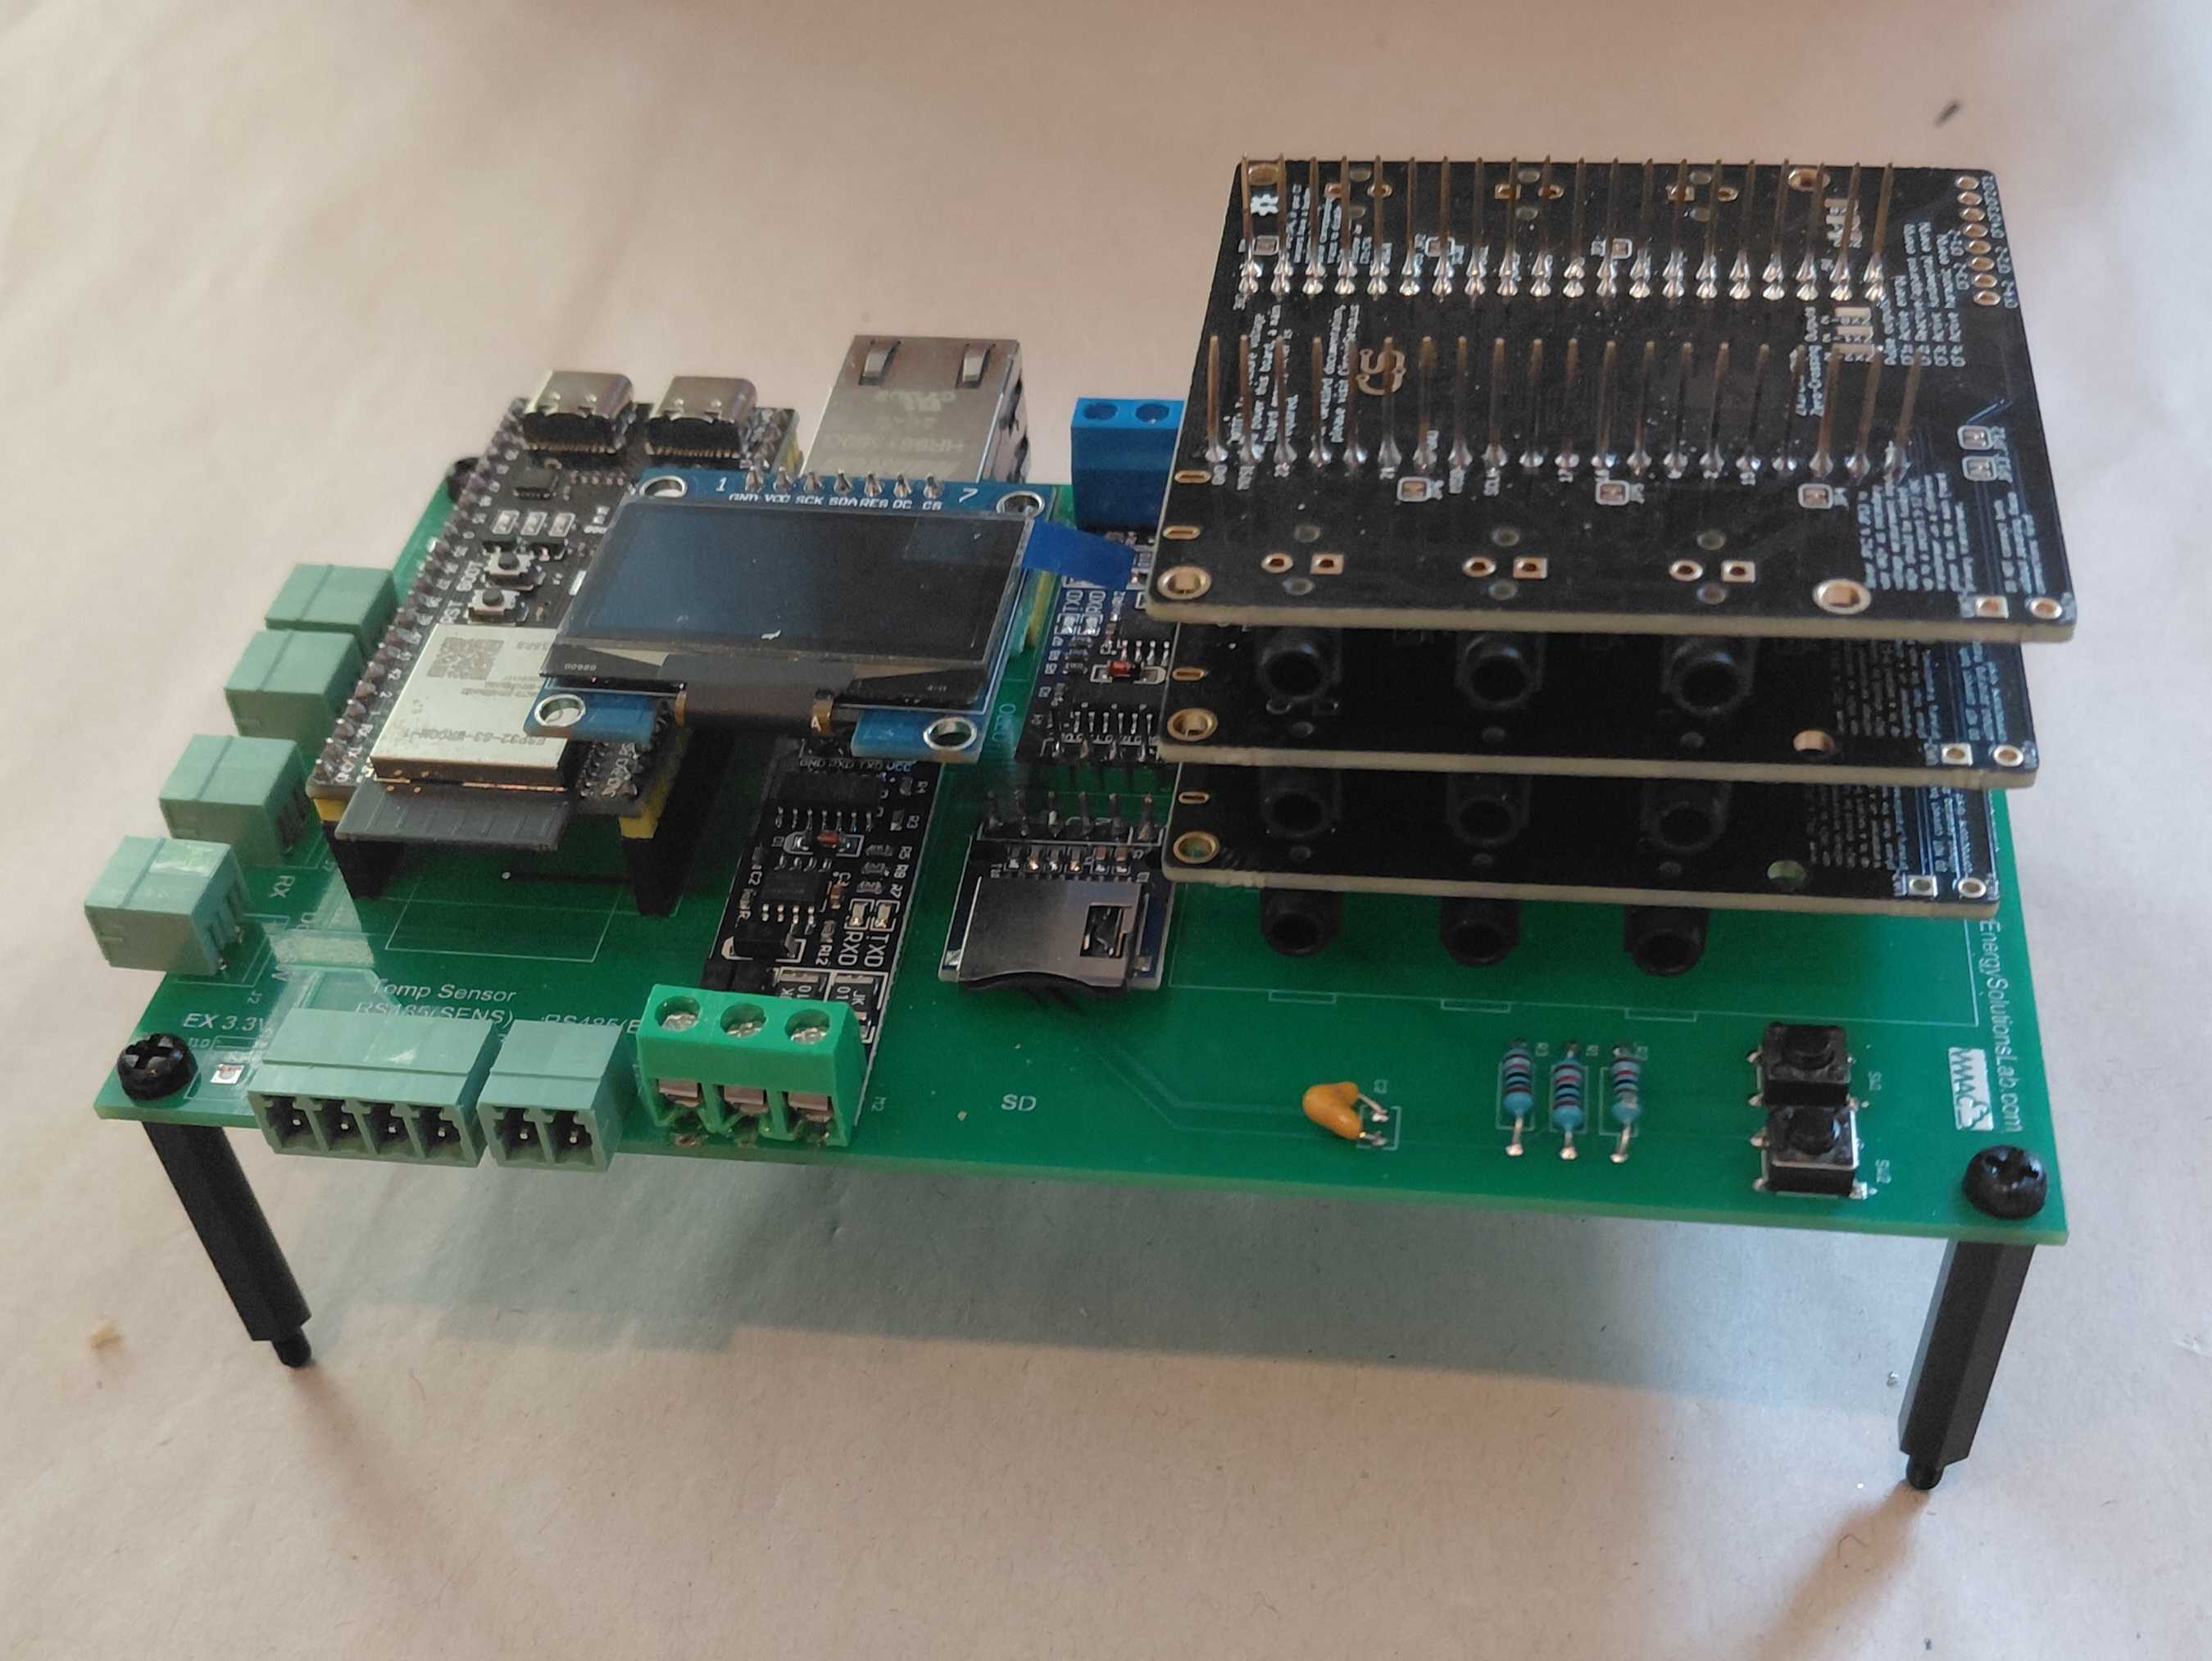
\includegraphics[width=0.96\linewidth]{street-ems.jpg}\end{center}}{%
  \begin{center}\setlength{\fboxsep}{0pt}\fcolorbox{tpgray}{tplight}{%
    \parbox[c][4.2cm][c]{0.94\linewidth}{\centering\color{tpgray}\itshape[ Product image: STREET-EMS / NESL 886B board ]}}\end{center}}

\vspace{7pt}
{\small
Designing a village minigrid? \textbf{STREET-EMS} is the open-source feeder controller for the
integration engineer building the \textbf{street pedestal cabinet} --- coordinating breakers and
contactors, metering each branch, and balancing distributed generation across the low-voltage
feeder. Front-of-meter, peer-to-peer, and autonomous at the edge.

\smallskip
\textbf{\color{tpdark}What Sets STREET-EMS Apart:}
\begin{arrows}
\item \textbf{Cabinet-Ready Control} : drives contactors and breaker coordination from an
onboard relay plus an 8-channel I\textsuperscript{2}C SSR expansion bank for per-branch switching.
\item \textbf{Open \& Vendor-Agnostic} : built on the open-source meshEMS stack; integrates
existing meters and DERs over Modbus, with no proprietary lock-in.
\item \textbf{Edge-Native Balancing} : feeder metering and load balancing run locally on a
dual-core edge MCU, with no dependence on cloud or central SCADA.
\item \textbf{Open-Source Hardware} : released under CERN-OHL-S v2 --- schematics, board files
and firmware published on GitHub (STREET-EMS).
\item \textbf{Field-Serviceable} : built from open, off-the-shelf commodity modules, snap-in
mounted for fast in-country assembly and repair.
\end{arrows}

\smallskip
From a single street pedestal, STREET-EMS meters every branch, switches loads via contactors,
and coordinates DERs --- bringing intelligent, balanced power to the village minigrid feeder.
}
\end{minipage}\hfill
\begin{minipage}[t]{0.37\textwidth}
\begin{featbox}{Intelligent}
\begin{arrows}
\item Multi-branch metrology: V, I, P, Q, PF, import/export kWh
\item Per-channel kW / kWh trip rules for load shedding
\item Roadmap: SIP energy-session admission
\end{arrows}
\end{featbox}
\vspace{7pt}
\begin{featbox}{Interoperable}
\begin{arrows}
\item 2$\times$ RS-485 (Modbus) + CAN 2.0
\item 8-ch I\textsuperscript{2}C SSR for contactors / breakers
\item WiFi / BLE \& wired Ethernet
\end{arrows}
\end{featbox}
\vspace{7pt}
\begin{featbox}{Resilient}
\begin{arrows}
\item Full edge autonomy without backhaul
\item Onboard + expansion relay control
\item microSD logging \sep OLED status
\end{arrows}
\end{featbox}
\end{minipage}

\vspace{11pt}
\setlength{\fboxsep}{6pt}%
\colorbox{tpdark}{\makebox[\dimexpr\textwidth-2\fboxsep][l]{%
\small\color{white}\textbf{New Energy Solutions Lab}\sep NewEnergySolutionsLab.com%
\hfill An NESL product for 10Power \sep Clean Growth.}}

% ===================== PAGE 2 : SPECIFICATIONS =====================
\clearpage
\thispagestyle{fancy}

{\fontsize{18}{20}\selectfont\bfseries\color{tpdark}Product Specifications}\hfill
\IfFileExists{TEN-POWER-LOGO-1.png}{\raisebox{-0.28\height}{
\includegraphics[height=0.72cm]{TEN-POWER-LOGO-1.png}}}{\footnotesize\textcolor{tpgray}{STREET-EMS}}\\[3pt]
\textcolor{tporange}{\rule{\textwidth}{1.5pt}}
\vspace{5pt}

{\small
\renewcommand{\arraystretch}{1.1}
\setlength{\tabcolsep}{6pt}
\begin{tabularx}{\textwidth}{@{}>{\bfseries\color{tpdark}\raggedright\arraybackslash}p{0.30\textwidth} >{\color{tpdark}\arraybackslash}X@{}}
\spechead{PRODUCT}
Product name & STREET-EMS (10Power X-EMS, supplied by NESL) \\
Model / PCB & NESL EMS Controller PCB 886B \\
Firmware & meshEMS / OpenAMI metering (open source, $\sim$50k LOC middleware) \\
License \& source & Hardware: CERN-OHL-S v2 \sep Repository: GitHub, STREET-EMS \\
Serviceability & Open, off-the-shelf commodity modules \sep snap-in mounted for fast in-country assembly and repair \\
\addlinespace[2pt]
\spechead{COMPUTE}
Processor & Dual-core 32-bit MCU @ 240 MHz \sep WiFi + Bluetooth LE \\
Memory & 16 MB Flash + 8 MB PSRAM \\
\addlinespace[2pt]
\spechead{ASSET COMMUNICATION}
Serial buses & 2$\times$ RS-485 Modbus: EVC + DTM/sensor ports \sep 1$\times$ CAN 2.0 \\
On-board metering & SPI poly-phase metering, up to 6 CT channels \sep V, I, P, Q, PF, freq \\
Local I/O & 2$\times$ onboard SSR \sep door-switch input \sep 2 analog buttons \\
\addlinespace[2pt]
\spechead{SUPPORTED MODULES \& SENSORS (out of the box)}
Energy meters (Modbus) & Single-phase Modbus energy meters \sep import/export kWh \\
Relay expansion & 8-channel I\textsuperscript{2}C solid-state relay (SSR) bank \sep per-channel kW / kWh trip rules \\
Environment sensor & Temperature / humidity sensor (Modbus) \\
DER interoperability & SunSpec models 1 / 11 / 213 \sep CAN 2.0 \\
\addlinespace[2pt]
\spechead{NETWORKING}
LAN & 10/100 Ethernet \sep RJ45 \\
Wireless & WiFi 802.11 b/g/n \sep Bluetooth 5 LE \\
\addlinespace[2pt]
\spechead{DISPLAY \& STORAGE}
Display \& storage & 1.3 in OLED display \sep microSD card slot \\
\addlinespace[2pt]
\spechead{POWER \& ENCLOSURE}
Operating voltage & 5 V DC --- USB-C or screw terminals \sep or 4.5\,--\,20 V DC \sep or 8\,--\,12 V AC (SELV) \\
Power / dimensions & 85 $\times$ 55 mm \sep or Raspberry Pi HAT form factor \\
\addlinespace[2pt]
\spechead{STANDARDS \& POSITIONING}
Grid position & Front-of-meter (FTM) \sep LV feeder \sep street pedestal cabinet \\
Target standards & IEEE ISV (front-of-meter feeder) \sep OpenAMI metrology \\
Capabilities & Peer-to-peer DER \& feeder balancing \sep contactor / breaker switching \\
\end{tabularx}}

\vspace{8pt}
{\footnotesize\textcolor{tpgray}{\itshape Customizable with added hardware modules and open or licensed code stacks.
STREET-EMS is an open-source X-EMS product supplied by New Energy Solutions Lab for 10Power.}}




\end{document}
